% ==== Colores estilo TAB10 ====
\definecolor{accblue}{RGB}{31,119,180}    % TEκ_α (azul)
\definecolor{accorange}{RGB}{255,127,14}  % TEKTE-Net Gaussian (naranja)
\definecolor{accgreen}{RGB}{44,160,44}    % TEKTE-Net RQ (verde)

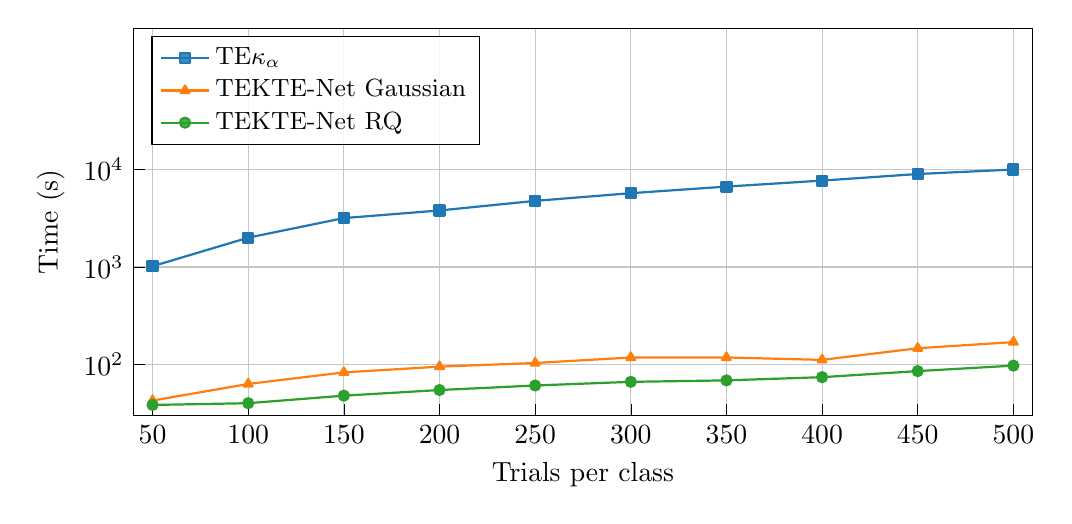
\begin{tikzpicture}
  \begin{axis}[
    width=13cm,
    height=6.5cm,
    xlabel={Trials per class},
    ylabel={Time (s)},
    xmin=40, xmax=510,
    ymin=30, ymax=45000,
    ymode=log,
    log basis y=10,
    xtick={50,100,...,500},
    ytick={1e2,1e3,1e4},
    tick pos=bottom,
    grid=both,
    yminorgrids=false,
    ymajorgrids=true,
    major grid style={line width=0.4pt, draw=gray!45},
    minor grid style={line width=0.3pt, draw=gray!30},
    tick align=inside,
    tick style={black},
    % ---- clave: crear espacio arriba sin que se salga la leyenda ----
    enlarge y limits={upper, value=0.25},
    legend style={
      at={(axis description cs:0.02,0.98)}, % <-- ahora SI queda dentro
      anchor=north west,
      draw=black,
      fill=white,
      fill opacity=0.85, text opacity=1,
      font=\small,
      nodes={align=left}
    },
    legend cell align=left,
    every axis plot/.append style={thick},
    line join=round
  ]
    % --- TEkappa_alpha ---
    \addplot[
      color=accblue,
      mark=square*,
      mark size=1.8pt
    ] coordinates {
      (50,  1017.37)
      (100, 1996.13)
      (150, 3169.36)
      (200, 3793.15)
      (250, 4757.60)
      (300, 5704.49)
      (350, 6665.44)
      (400, 7677.96)
      (450, 8968.81)
      (500, 9969.30)
    };
    \addlegendentry{TE$\kappa_\alpha$}
    % --- TEKTE-Net Gaussian ---
    \addplot[
      color=accorange,
      mark=triangle*,
      mark size=1.8pt
    ] coordinates {
      (50,  42.69)
      (100, 63.17)
      (150, 83.03)
      (200, 95.08)
      (250, 103.63)
      (300, 117.95)
      (350, 118.11)
      (400, 111.52)
      (450, 146.85)
      (500, 169.74)
    };
    \addlegendentry{TEKTE-Net Gaussian}
    % --- TEKTE-Net RQ ---
    \addplot[
      color=accgreen,
      mark=*,
      mark size=1.8pt
    ] coordinates {
      (50,  38.49)
      (100, 40.13)
      (150, 47.92)
      (200, 54.74)
      (250, 60.94)
      (300, 66.43)
      (350, 68.73)
      (400, 74.16)
      (450, 85.57)
      (500, 97.39)
    };
    \addlegendentry{TEKTE-Net RQ}
  \end{axis}
\end{tikzpicture}
